\section{Reverse Engineering}
Abstraktionsniveau
Assembler als Haupt-Programmiersprache für Softwareprojekte hat auf Grund der großen Verbreitung einer Vielzahl von Hochsprachen, mit samt deren Vorteilen wie höheres Abstraktionsniveau, umfangreiche Werkzeuge, hohe Portierbarkeit und Wirtschaftlichkeit von Wartung und Kollaboration in Teams, stark an Bedeutung verloren. Auch sind die Hauptstärken von Assembler Schnelligkeit und geringe Codegröße durch das Aufkommen hochoptimierender Compiler und dem exponentiellem Wachstum von Prozessorleistung und Speicherkapazitäten in den Hintergrund getreten.

Doch auch ohne das heute noch viel direkt in Assembler programmiert wird ist die Kenntnis der Sprache unverzichtbar für das sogenannte \emph{Reverse Engineering}. Damit bezeichnet man im Software-Kontext die Disassemblierung und Analyse von binärem Programmcode, also allem übersetzten, ausführbaren Code eines Computers. Man kann es sich als ein "Zurückgehen im Entwicklungsprozess" vorstellen.\cite{Warden1992}

Dies kann aus vielerlei Motivation möglich sein:
\begin{itemize}
\item Debugging von Compilerfehlern oder Programmen ohne Quelltext
\item Schadcode-Analyse z.B. in der Antivirenindustrie
\item Forensische Analyse nach einer Sicherheitskompromitierung ("Hacker-Angriff")
\item Sicherheitslücken suchen und aufdecken durch Sicherheitsforscher
\item Umgehung von Kopierschutz durch Entwickeln von \emph{Cracks} (binäre Patches)
\item Umgehung von Kopierschutz durch \emph{Keygeneratoren} – Analyse und Nachbau des Lizensierungsschemas einer kommerziellen Anwendung
\item Analyse, Umgehung oder Entfernung von \emph{Digital Rights Management}
\end{itemize}

Die Vorgehensweise soll am Beispiel der Schadcode-Analyse kurz beschrieben werden: ein Antivirenhersteller und unabhängiges Forscherteam enthält unbekannten Virencode durch Einsendung eines Tipgebers dem Einsammeln von infizierten Dateien auf speziellen "Locksystemen" (\emph{Honey-pots}). Dieser auch als \emph{Sample} bezeichnete Binärcode wird in einem Disassembler geladen und zunächst statisch analysiert. Neben dem Assembler-Listing und vorinitialisierten Daten wie Strings und Tabellen, erhält man oft auch Informationen Programmelemente höherer Abstraktionslevel wie Structs, Klassen und deren Methoden und Funktions- und Variablennamen (wenn sie Zwecken des Ausführens oder Debuggens erforderlich waren bzw. absichtlich in das Programm kompiliert wurden).
Oft lassen sich auch Flussdiagramme und Aktivierungsbäume von Funktionsaufrufen automatisch generieren.

\begin{figure}[h]
  \begin{center}
	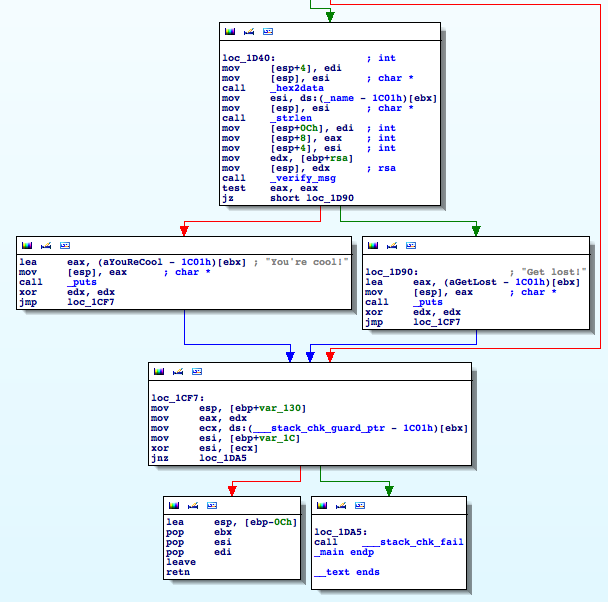
\includegraphics[width=0.85\textwidth]{IDA-pro-flowdiagram.png}
  \end{center}
  \caption{Flussdiagramm eines Programmsegments in IDA Pro}
\end{figure}

Da diese Disassembler oft auch auf Seiten der Virenentwicklers zum Grundwerkzeug gehören werden in der Praxis oft Verschleierungs- oder sogar Verschlüsselungs-Techniken eingesetzt, die statische Code-Analyse erschweren oder unmöglich machen. Die meisten Disassembler sind aber auch Debugger und erlauben die Analyse zur Laufzeit – bei Schadcode meist in einer gesicherte Laborumgebung. Ein \emph{Trace} durch den Programmablauf hinterlässt dann eine Spur des tatsächlich ausgeführten, aktiven Codes.

Das Umgehen von Software-Sicherungen zum Kopierschutz oder Passwortabfragen ist ein anderes Einsatzfeld von Reverse-Engineering-Techniken im legalen Graubereich – Patent-, Eigentums- und Urheberechtsgesetze werden oft verletzt. Es gibt jedoch auch Enthusiasten, die \emph{Cracking} aus "sportlichen" Gründen betreiben und von den facettenreichen Fähigkeiten fasziniert sind die dazu häufig nötig sind. Ein legaler Weg sind sogenannte \emph{Crackme}, kleine Programme die von anderen "\emph{Reversern}" geschrieben wurden um sich gegenseitig auszuprobieren oder herauszufordern.

Ein weiteres Gebiet in dem Assemblercode geschrieben und gelesen werden, muss ist das Entwickeln bzw. Analysieren von \emph{Exploits}. So bezeichnet man kurze Programme zum aktiven Ausnutzen von Sicherheitslücken. Meist geht es dabei darum subversiv, eigenen Code in fremde Computersysteme einzuschleusen und sich nicht-autorisierten Zugang zu verschaffen. Assembler taucht hier meist in Form von \emph{Shellcode} auf. Code der so heißt, da er in der Regel zum Starten einer privilegierten, fernsteuerbaren Shell auf dem Fremdsystem eingeschleust wird. Der Shellcode wird in Form einer mit falscher Absicht zusammengesetzten Dateneingabe eingebracht, auf die die entgegennehmende Software fehlerhaft reagiert. Der Shellcode befindet sich dann schon auf dem Stack oder Heap des anfälligen Programms und muss geschickt unter Ausnutzung der Sicherheitslücke angesprungen werden. Gute Assemblerkentnisse sind für den Exploit-Programmierer Voraussetzung. Die Motivationen sind wiederum vielschichtig und reichen von wissenschaftlichem Forschungsgeist über persönlichen Ehrgeiz bis zu kriminelle Absichten.
